\documentclass[xcolor={rgb}]{beamer}
\usepackage[labelformat=empty]{caption}

\newcommand{\pitem}{\pause\item}
\usetheme{metropolis}

\newcommand{\img}[3]{
	\only<#1>{
		\begin{figure}
			\includegraphics[width=\textwidth]{#2}
			\caption{#3}
		\end{figure}
	}
}

\newcounter{_i}
\newcommand{\starcounting}{\setcounter{_i}{2}}
\newcommand{\simg}[2]{
	\stepcounter{_i}
	\img{\value{_i}}{#1}{#2}
}

\newcommand\XOR{\mathbin{\char`\^}}

\author{Alireza Arzehgar}
\title{OpenBSD W\^{}X story}
\date{\today}

\begin{document}
	\begin{frame}[plain]
		\titlepage
	\end{frame}

	\begin{frame}{UNIX History}
		\begin{itemize}
			\pitem UNIX - 1969
			\pitem BSD - 1978
			\pitem NetBSD - 1993 (Founders: Chris, Theo, Adam, Charles)
			\pitem OpenBSD - 1995 (Founder: Theo)
		\end{itemize}
	\end{frame}

	\begin{frame}{How OpenBSD arised?}
		\begin{itemize}
			\pitem Theo De Raadt disagreed with NetBSD team.
			\pitem Theo goals
			\begin{itemize}
				\pitem Freedom
				\pitem Security
				\pitem Correctness
				\pitem Simplicity
			\end{itemize}
		\end{itemize}
	\end{frame}

	\begin{frame}{OpenBSD Culture}
		\begin{itemize}
			\pitem Conferences
			\pitem Papers
			\pitem Releases
			\pitem Hackathons
			\pitem Artworks
			\pitem Songs
		\end{itemize}
	\end{frame}

	\begin{frame}{3.3: Puff the Barbarian}
		\center
		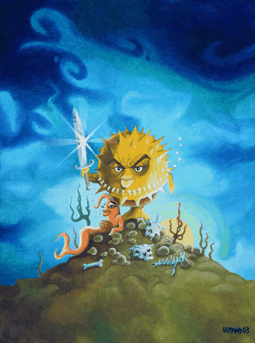
\includegraphics[height=0.9\textheight]{./assets/puff.png}
	\end{frame}

	\begin{frame}{W\^{}X}
		\begin{itemize}
			\pitem Memory Protection
			\pitem Buffer Overflow
			\pitem XOR
			\pitem Write or Execute
		\end{itemize}
	\end{frame}

	\begin{frame}{MMU}
		\begin{itemize}
			\pitem Help to kernel
			\pitem Memory Protection
			\pitem Virtual Memory
			\pitem per-page eXecute bit or Permission
		\end{itemize}
	\end{frame}

	\begin{frame}{OpenBSD drama}
		\begin{center}
		\Huge UltraSPARC III vs AMD Hammer
		\end{center}
	\end{frame}

	\begin{frame}{OpenBSD drama}
		\begin{center}
		\Huge Open to discussion
		\end{center}
	\end{frame}
\end{document}
